\documentclass[12pt]{article}
\usepackage[english]{babel}
\usepackage[utf8]{inputenc}
\usepackage{amsmath, amssymb, amsthm}
\usepackage{graphicx}
\usepackage{hyperref}
\usepackage{geometry}
\usepackage{xcolor}
\usepackage{tikz}

\setlength{\topmargin}{0pt}
\setlength{\headsep}{0pt}
\textheight = 600pt

\title{Graph Theory \\ Homework 1}
\author{Ben Kallus and Maddy LaPoint}
\date{Due Friday, February 5}

\begin{document}
\pagecolor{black}
\color{white}
\maketitle

\noindent{\bf 1.1}

    After reading Example 1.1, the next logical question to ask is whether it is possible to have all seven committees meet without conflict in the three time slots.
    This is possible since, for example, $c_1$, and $c_4$ can meet in the first time slot, $c_7$ and $c_3$ can meet in the second time slot, and $c_6$, $c_2$, and $c_5$ can meet in the third time slot.


\bigskip
\noindent{\bf 1.4}

    $G:$

    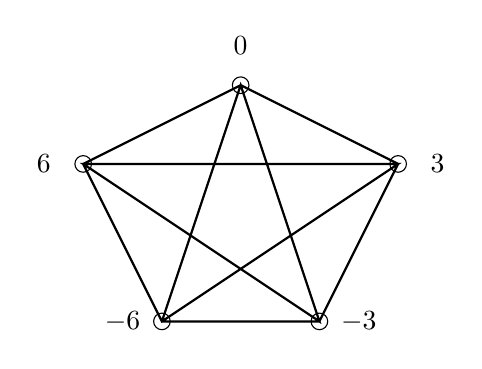
\begin{tikzpicture}
        %% vertices
        \draw[fill=white] (1,0) circle (3pt);
        \draw[fill=white] (3,0) circle (3pt);
        \draw[fill=white] (4,2) circle (3pt);
        \draw[fill=white] (2,3) circle (3pt);
        \draw[fill=white] (0,2) circle (3pt);
        %% vertex labels
        \node at (0.5,0) {$-6$};
        \node at (3.5,0) {$-3$};
        \node at (4.5,2) {$3$};
        \node at (2,3.5) {$0$};
        \node at (-0.5,2) {$6$};
        %% edges
        \draw[thick] (1,0) -- (3,0) -- (4,2) -- (2,3) -- (0,2) -- (1,0) -- (4,2) -- (0,2) -- (3,0) -- (2,3) -- (1,0);
    \end{tikzpicture}

\newpage
\noindent{\bf 1.6}
    
    $F:$
    \bigskip

    \newcommand{\cone}{(-.5,-.5)}
    \newcommand{\ctwo}{(1,-4)}
    \newcommand{\cthree}{(-1,-4)}
    \newcommand{\cfour}{(.5,-.5)}
    \newcommand{\cfive}{(-3,-2)}
    \newcommand{\csix}{(-3,0)}
    \newcommand{\cseven}{(.5,-1.5)}
    \newcommand{\ceight}{(-1,2)}
    \newcommand{\cnine}{(1,2)}
    \newcommand{\cten}{(-.5,-1.5)}
    \newcommand{\celeven}{(3,0)}
    \newcommand{\ctwelve}{(3,-2)}

    \begin{tikzpicture}
        %% vertices
        \draw[fill=white] \cone circle (3pt);
        \draw[fill=white] \ctwo circle (3pt);
        \draw[fill=white] \cthree circle (3pt);
        \draw[fill=white] \cfour circle (3pt);
        \draw[fill=white] \cfive circle (3pt);
        \draw[fill=white] \csix circle (3pt);
        \draw[fill=white] \cseven circle (3pt);
        \draw[fill=white] \ceight circle (3pt);
        \draw[fill=white] \cnine circle (3pt);
        \draw[fill=white] \cten circle (3pt);
        \draw[fill=white] \celeven circle (3pt);
        \draw[fill=white] \ctwelve circle (3pt);
        %% vertex labels
        \node at (-.25,-.5-.25) {$c_1$};
        \node at (1,-4+.5) {$c_2$};
        \node at (-1,-4+.5) {$c_3$};
        \node at (.25,-.5-.25) {$c_4$};
        \node at (-3,-2+.5) {$c_5$};
        \node at (-3,0+.5) {$c_6$};
        \node at (.25,-1.5+.25) {$c_7$};
        \node at (-1,2+.5) {$c_8$};
        \node at (1,2+.5) {$c_9$};
        \node at (-.25,-1.5+.25) {$c_{10}$};
        \node at (3,0+.5) {$c_{11}$};
        \node at (3,-2+.5) {$c_{12}$};
        %% edges
        \draw[thick] \cone -- \cfive -- \cten -- \ctwo -- \cseven -- \cthree -- \cten -- \csix -- \cone -- \ceight -- \cfour -- \cnine -- \cone;
        \draw[thick] \cfour -- \celeven -- \cseven -- \ctwelve -- \cfour;
    \end{tikzpicture}

\end{document}